\documentclass[11pt]{report}
\usepackage{graphicx}
\usepackage{tabularx}
\usepackage{graphicx}
\usepackage[margin=0.5in]{geometry}
\usepackage{listings,xcolor}
\lstset{
    string=[s]{"}{"},
    stringstyle=\color{blue},
    comment=[l]{:},
    commentstyle=\color{black},
    breaklines=true,
}
\PassOptionsToPackage{hyphens}{url}\usepackage{hyperref}
\begin{document}

\title{Assignment 5}
\author{Joshua Graham}

\maketitle
\pagebreak
\begin{abstract}
All Scripts used in the assignment can be found in the A5 folder, if needed.

\end{abstract}
\section{Problem 1}
	Question 1 was only a difficult question for me due to me misunderstanding the task, and what tools I had. After 3 hours of attempting to create the graph manually, I reread the source material listed and found that several of the steps could be done using the networkx package.The code I used is below, but can also be found in the file graph.py.
	

\begin{lstlisting}[language=Python]
import networkx
from matplotlib import pylab

G = networkx.karate_club_graph()
pos = networkx.spring_layout(G)
c = networkx.connected_component_subgraphs(G)
iterCount=0
print("Iteration: ", iterCount)
output = "graph" + format(iterCount, '02d') + ".png"
pylab.figure()
networkx.draw_networkx(G, pos)
pylab.savefig(output)
pylab.close()
while (len(list(c)) == 1):
    #G.remove_edge(*edge_to_remove(G))
    hold = networkx.edge_betweenness_centrality(G)
    curr = hold.items()
    currSorted = sorted(curr,key=lambda x:x[1], reverse = True)
    G.remove_edge(*currSorted[0][0])
    c = networkx.connected_component_subgraphs(G)
    pos = networkx.spring_layout(G)
    iterCount += 1
    output = "graph" + format(iterCount, '02d') + ".png"
    print("Iteration: ", iterCount)
    pylab.figure()
    networkx.draw_networkx(G, pos)
    pylab.savefig(output)
    pylab.close()
pylab.figure()
c = networkx.connected_component_subgraphs(G)
pos = networkx.spring_layout(G)
networkx.draw_networkx(G, pos)
networkx.draw_networkx_nodes(G, pos, nodelist=[0, 1, 3, 4, 5, 6, 7, 10, 11, 12, 13, 16, 17, 19, 21], node_color='b')
pylab.savefig("final.png")
pylab.close()


\end{lstlisting}
\pagebreak

The intial graph is posted on the left, and the result is on the right. From the examples listed below, as far as I can tell with the expection of a few nodes, the algorithm correctly sperated the two groups to closely match the split of the club. There are one or two differences between the list and the actual result. I believe this falls under a margin of error, as the rest of the graph closely matches the intended result. 

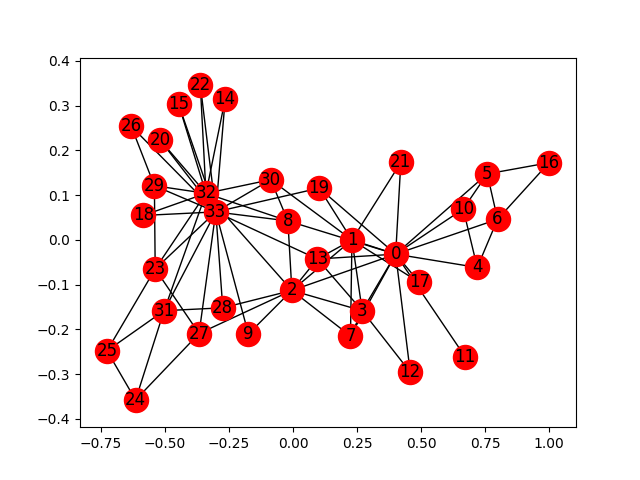
\includegraphics[scale=0.5]{graph01.png}
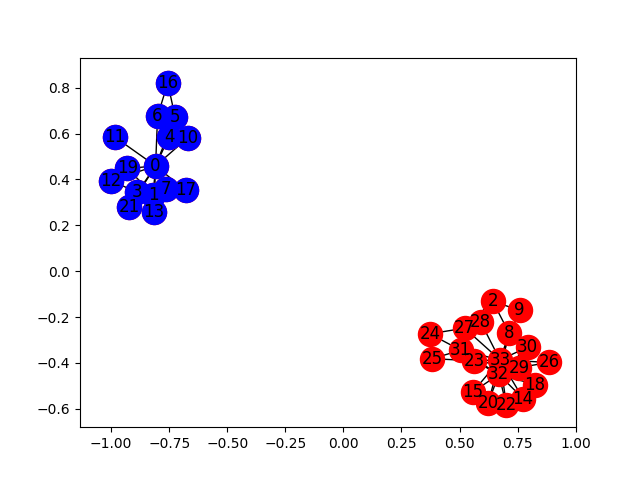
\includegraphics[scale=0.5]{final.png}


\end{document}